\chapter{Regressione lineare}


\section{Exercise 1}
Rilevare e stimare eventuali trend su ognuna delle tre variabili nmail, byte rec e byte sent, utilizzando modelli regressivi lineari semplici, parametrici e/o non parametrici


La normalità dei residui è una condizione necessaria per l'utilizzo di una regressione lineare come modello, motivo per il quale per entrambi i dataset è stata inizialmente svolta un'analisi sulla normalità dei residui ottenuti in seguito a una stima lineare di ogni colonna rispetto alle osservazioni.


\subsection{EXP1}
È possibile notare dal diagramma quantile quantile e dal test di \textit{Anderson-Darling} la non normalità della distribuzione dei residui per tutte e tre le variabili (\cref{fig:4_ex1_traccia}).
Si è quindi proceduto con il test di \textit{Mann Kendall} per verificare la presenza di trend monotoni, e in caso positivo è stato calcolato lo \textit{slope} sia con la procedura di \textit{Theil-Sen}. Nei grafici che seguono è possibile notare in rosso i risultati ottenuti con \textit{Theil-Sen}, mentre in verde il risultato ottenuto con il metodo dei quadrati minimi, inserito come base di confronto.

\begin{figure}[H]
    \centering
    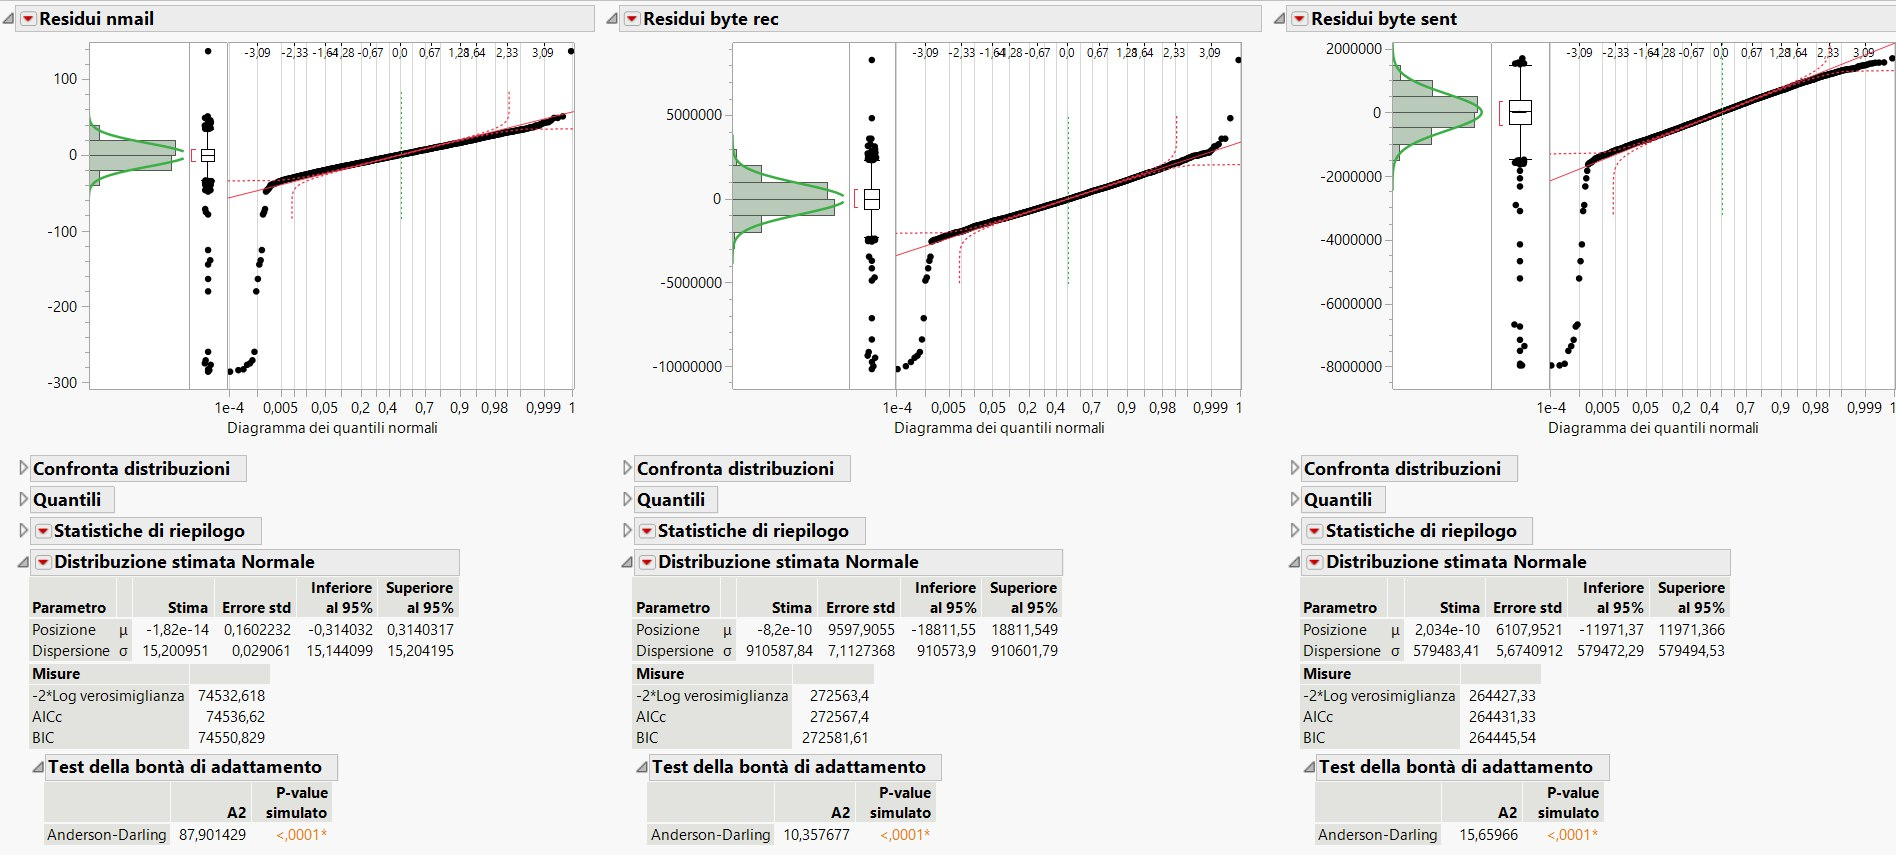
\includegraphics[width=\textwidth]{img/ch4/exp1norm.jpg}
    \caption{Test normalità residui}
    \label{fig:4_ex1_traccia}
\end{figure}

\paragraph{Analisi \textit{nmail}}
Il risultato del test di \textit{Man-Kendall} mostra che non è possibile determinare la presenza di un \textit{trend} ($pvalue=0.7163$). Si noti che l'intervallo di confidenza individuato con il test di Theil-Sen $(0.0;0.0)$ include il valore $0$. 

\begin{figure}[H]
    \centering
    \includegraphics[width=\textwidth]{img/ch4/exp1.1.pdf}
    \caption{Trend nmail per EXP1}
\end{figure}


\paragraph{Analisi \textit{byte rec}}
Il risultato del test di Man Kendall mostra che non è possibile determinare la presenza di un \textit{trend} ($pvalue=0.2001$). Si noti che l'intervallo di confidenza individuato con il test di Theil-Sen $(-11.5115;2.4138)$ include il valore $0$. 

\begin{figure}[H]
    \centering
    \includegraphics[width=\textwidth]{img/ch4/exp1.2.pdf}
    \caption{Trend byte rec}
    \label{fig:ex1_traccia}
\end{figure}


\paragraph{Analisi \textit{byte sent}}
Il risultato del test di Man Kendall mostra la presenza di un \textit{trend} decrescente ($pvalue=0.0434$). Il test di Theil-Sen produce una retta:

\begin{equation}
    y = -4.5147 \cdot x + 9959247.5279
\end{equation}

L'intervallo di confidenza (calcolato al $95\%$)  del coefficiente angolare è\\ $(-8.8910;-0.1306)$.

\begin{figure}[H]
    \centering
    \includegraphics[width=\textwidth]{img/ch4/exp1.3.pdf}
    \caption{Trend byte sent}
\end{figure}


\newpage
\subsection{EXP2}
Anche in questo caso è possibile notare dal diagramma quantile quantile e dal test di \textit{Anderson-Darlnig} la non normalità della distribuzione dei residui per tutte e tre le variabili (\cref{fig:4_ex2_traccia}).
Si è quindi proceduto con il test di \textit{Mann Kendall} per verificare la presenza di trend monotoni, e in caso positivo è stato calcolato lo slope con la procedura di \textit{Theil-Sen}.

\begin{figure}[H]
    \centering
    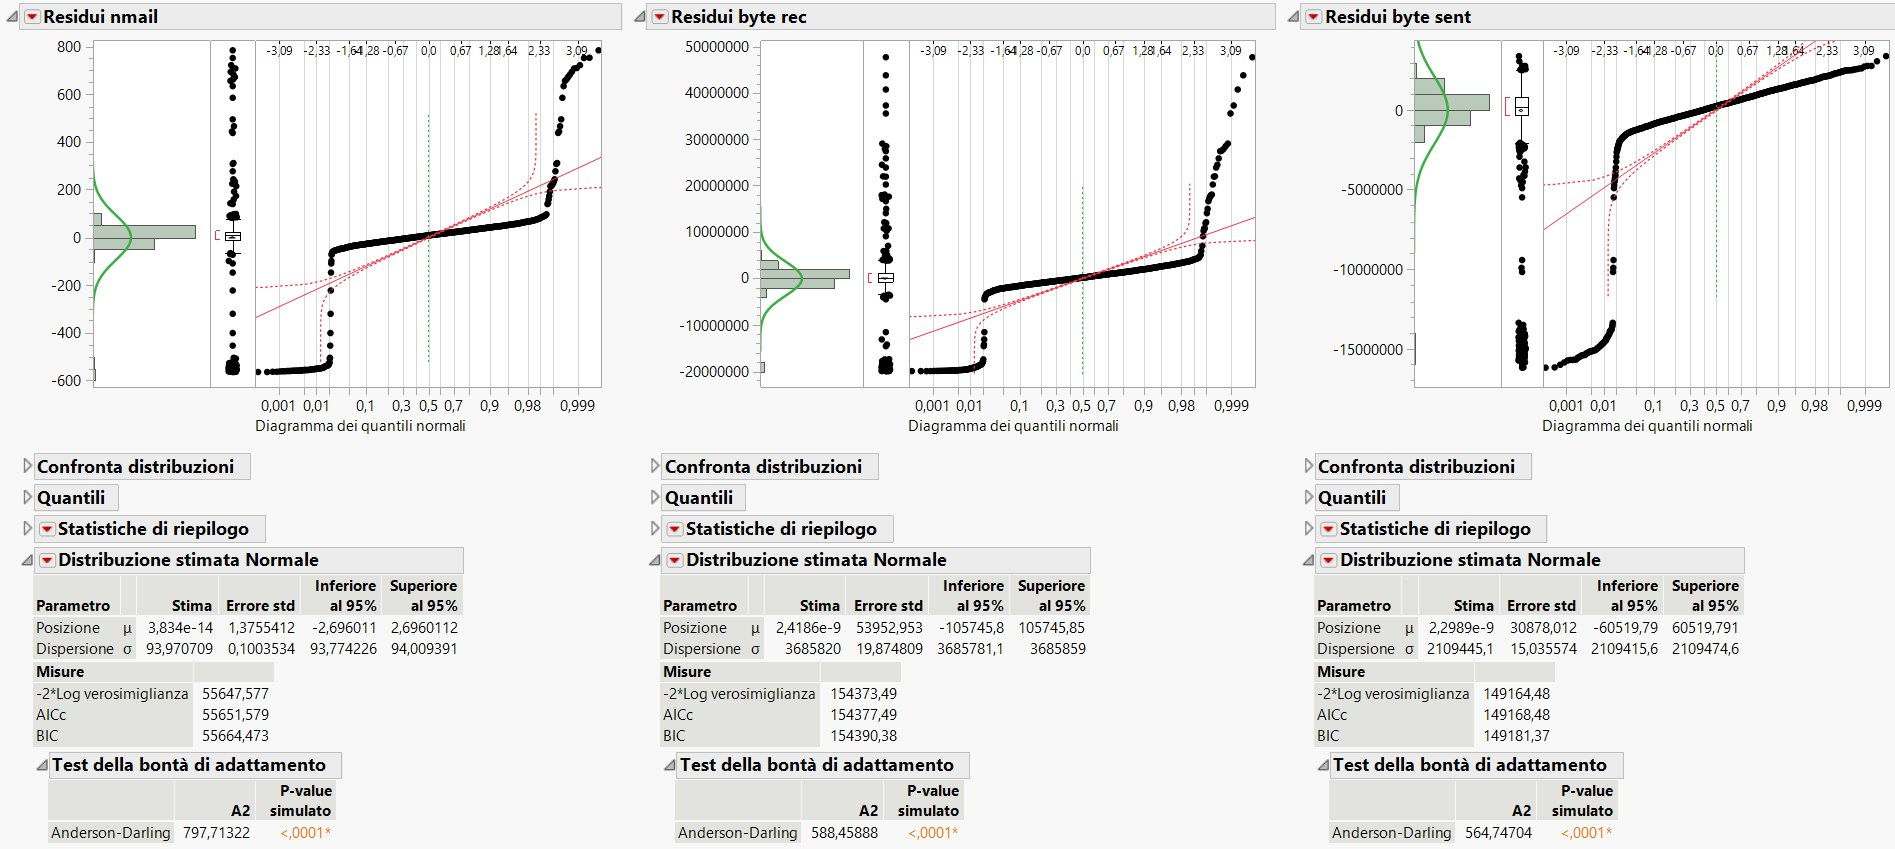
\includegraphics[width=\textwidth]{img/ch4/exp2.jpeg}
    \caption{Test normalità residui}
    \label{fig:4_ex2_traccia}
\end{figure}

\paragraph{Analisi \textit{nmail}}
Il risultato del test di Man Kendall mostra la presenza di un \textit{trend} decrescente ($pvalue=0.0138$). Il test di Theil-Sen produce una retta:

\begin{equation}
    y = -0.0005 x + 592.3936
\end{equation}

L'intervallo di confidenza (calcolato al $95\%$)  del coefficiente angolare è\\ $(-0.0011;0.0)$.

\begin{figure}[H]
    \centering
    \includegraphics[width=\textwidth]{img/ch4/exp2.1.pdf}
    \caption{Trend nmail per EXP2}
\end{figure}


\paragraph{Analisi \textit{byte rec}}
Il risultato del test di Man Kendall mostra la presenza di un \textit{trend} decrescente ($pvalue=0.0012$). Il test di Theil-Sen produce una retta:

\begin{equation}
    y = -48.2936 x + 20890131.9913
\end{equation}

L'intervallo di confidenza (calcolato al $95\%$) del coefficiente angolare è\\ $(-77.5477;-18.9931)$.

\begin{figure}[H]
    \centering
    \includegraphics[width=\textwidth]{img/ch4/exp2.2.pdf}
    \caption{Trend \textit{byte rec} EX1}
\end{figure}

\paragraph{Analisi \textit{byte sent}}
Il risultato del test di Man Kendall mostra la presenza di un \textit{trend} decrescente ($pvalue=5.8473\cdot 10^{-5}$). Il test di Theil-Sen produce una retta:
\begin{equation}
    y = -34.0630 x + 19903064.1005
\end{equation}

L'intervallo di confidenza (calcolato al $95\%$) del coefficiente angolare è\\ $(-50.6726;-17.3740)$.

\begin{figure}[H]
    \centering
    \includegraphics[width=\textwidth]{img/ch4/exp2.3.pdf}
    \caption{Trend \textit{byte sent} EX2}
\end{figure}

\newpage
\section{Exercise 2}
Rilevare e stimare eventuali trend sulle 5 variabili utilizzando modelli regressivi lineari semplici, parametrici e/o non parametrici. Farlo per i tre dataset os1, os2 e os3.
Confrontare i trend individuati nei tre dataset.

Per tutti e tre i dataset è stata inizialmente svolta un'analisi sulla normalità dei residui ottenuti in seguito a una stima lineare di ogni colonna rispetto al tempo di osservazione. 

\subsection{Sistema \textit{os1}}
È possibile notare dal diagramma quantile quantile e dal test di \textit{Anderson-Darling} la non normalità delle distribuzioni (\cref{fig:4_os1_traccia}).
Si è quindi proceduto con il test di \textit{Mann Kendall} per verificare la presenza di trend monotoni, e in caso positivo è stato calcolato lo slope con la procedura di \textit{Theil-Sen}.

\begin{figure}[H]
    \centering
    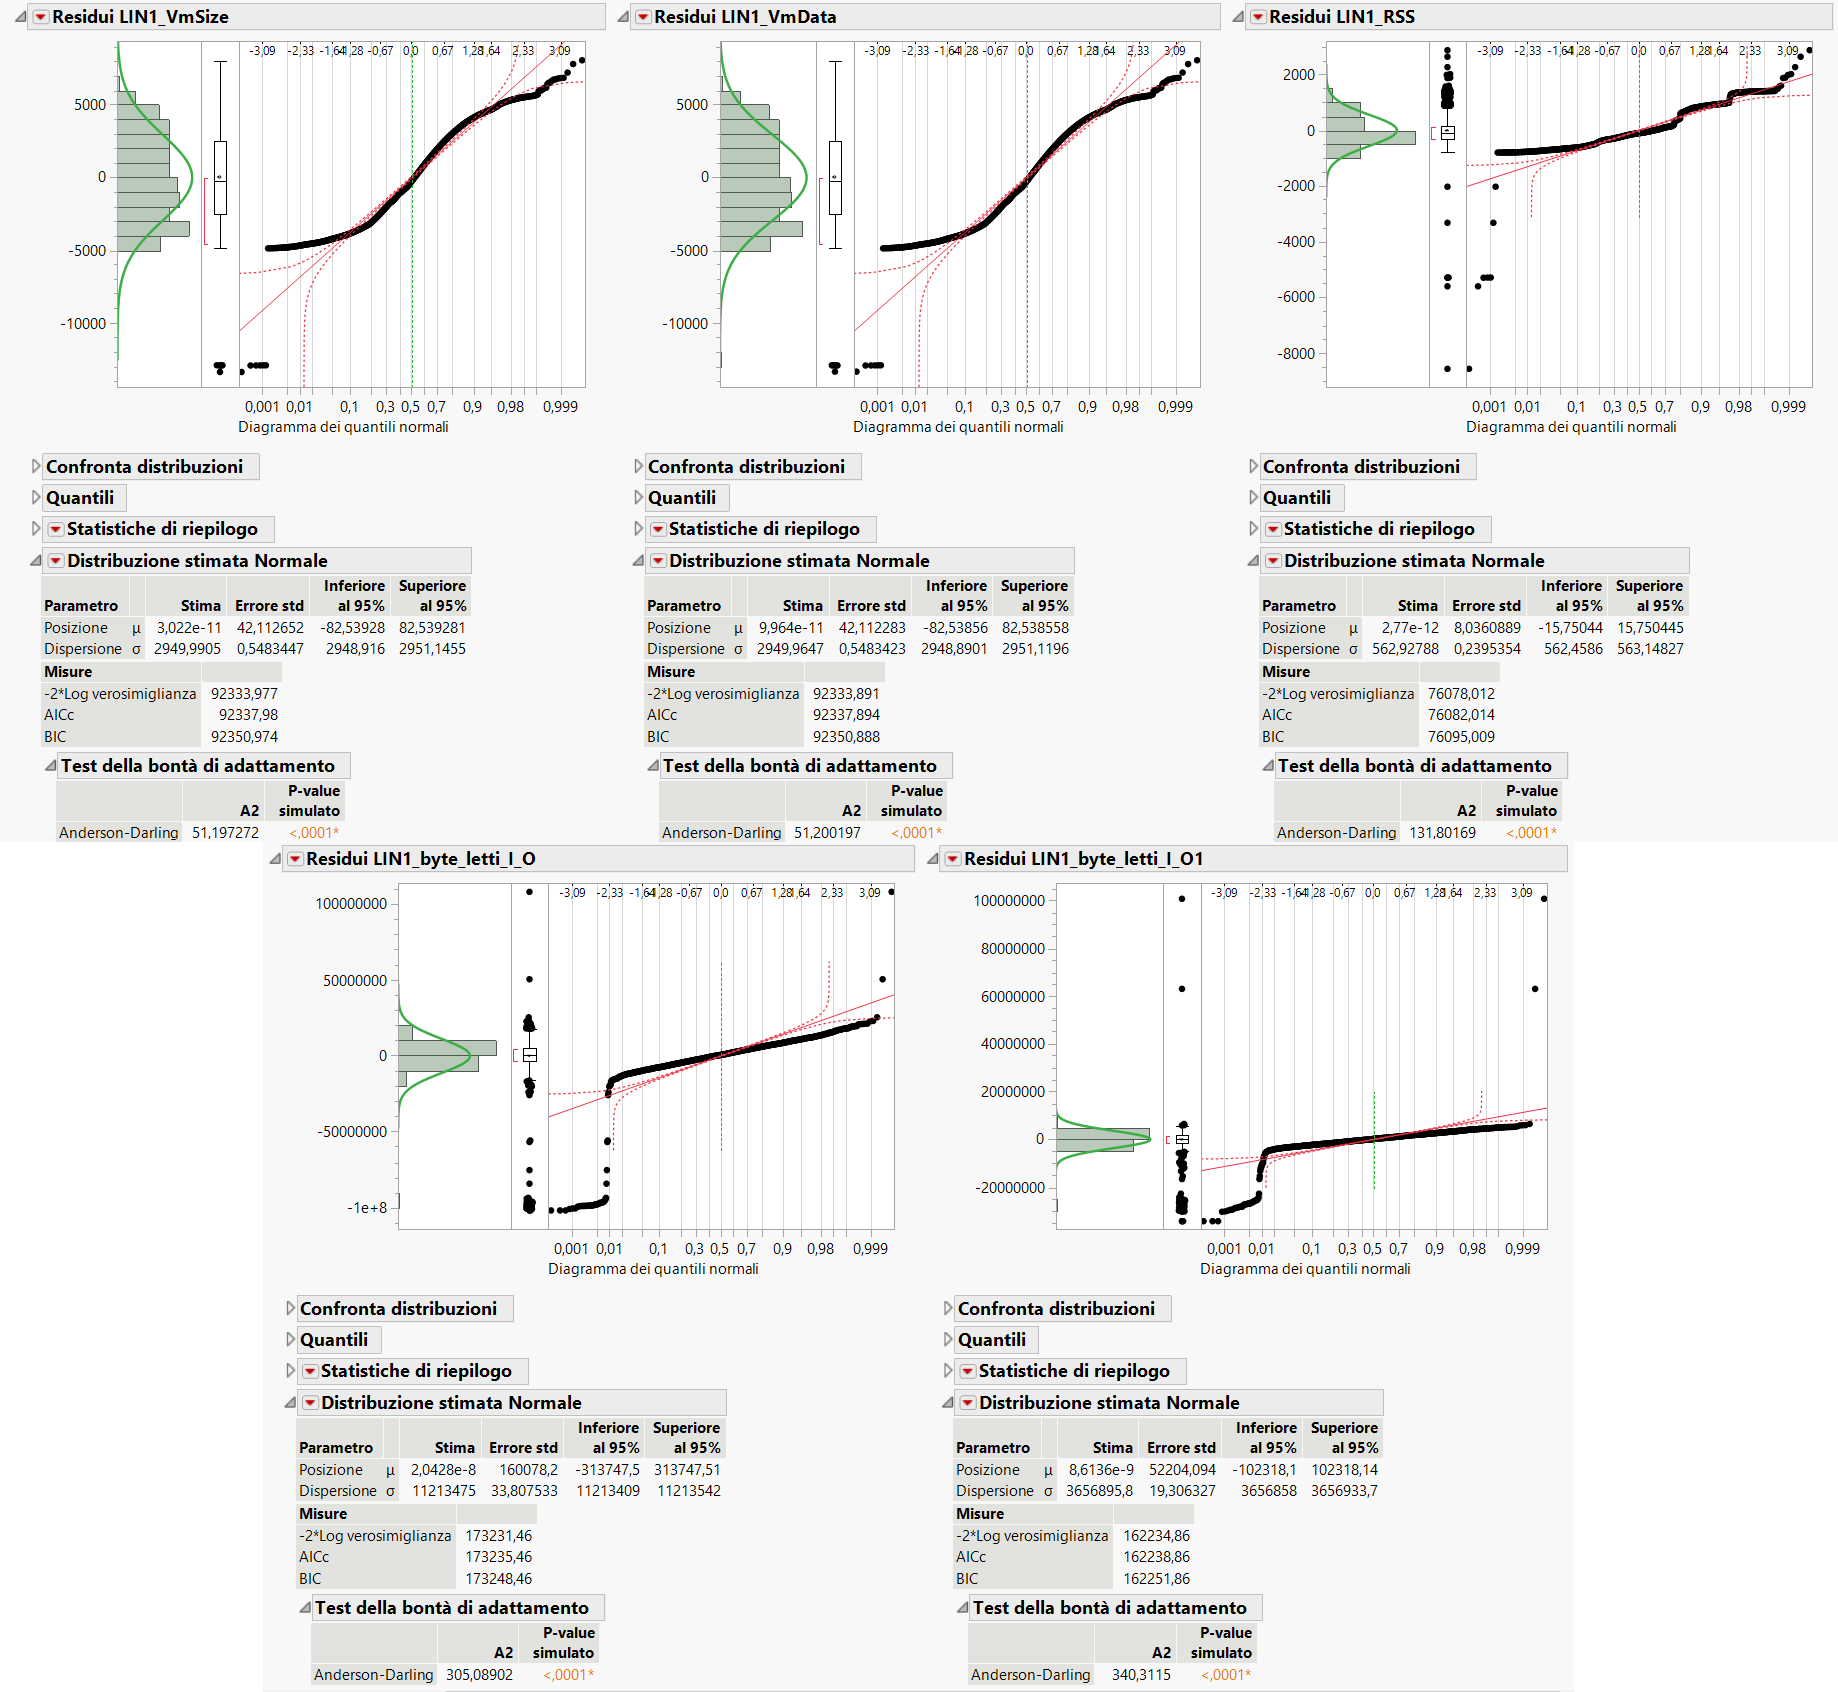
\includegraphics[width=\textwidth]{img/ch4/os1norm.png}
    \caption{Test normalità residui per $os1$}
    \label{fig:4_os1_traccia}
\end{figure}

\paragraph{LIN1 VmSize}
Il risultato del test di Man Kendall mostra la presenza di un \textit{trend} crescente ($pvalue=0.0$). Il test di Theil-Sen produce una retta:
\begin{equation}
    y = 0.03151 x + 738854.3947
\end{equation}

L'intervallo di confidenza (calcolato al $95\%$) del coefficiente angolare è\\ $(0.0307;0.0323)$.

\begin{figure}[H]
    \centering
    \includegraphics[width=\textwidth]{img/ch4/os1.1.pdf}
    \caption{Trend LIN1 VmSize}
\end{figure}

\paragraph{LIN1 VmData}
Il risultato del test di Man Kendall mostra la presenza di un \textit{trend} crescente ($pvalue=0.0$). Il test di Theil-Sen produce una retta:
\begin{equation}
    y = 0.0315 x + 670450.3948
\end{equation}

L'intervallo di confidenza (calcolato al $95\%$) del coefficiente angolare è\\ $(0.0307;0.0323)$.

\begin{figure}[H]
    \centering
    \includegraphics[width=\textwidth]{img/ch4/os1.2.pdf}
    \caption{Trend LIN1 VmData}
\end{figure}

\paragraph{LIN1 RSS}
Il risultato del test di Man Kendall mostra la presenza di un \textit{trend} crescente ($pvalue=0.0$). Il test di Theil-Sen produce una retta:
\begin{equation}
    y = 0.0049 x + 42428.8070
\end{equation}

L'intervallo di confidenza (calcolato al $95\%$) del coefficiente angolare è\\ $(0.00488;0.0050)$.

\begin{figure}[H]
    \centering
    \includegraphics[width=\textwidth]{img/ch4/os1.3.pdf}
    \caption{Trend LIN1 RSS}
\end{figure}

\paragraph{LIN1 byte letti IO}
Il risultato del test di Man Kendall mostra la presenza di un \textit{trend} crescente ($pvalue=0.0$). Il test di Theil-Sen produce una retta:
\begin{equation}
    y = 4.7375 x + 102763229.5031
\end{equation}

L'intervallo di confidenza (calcolato al $95\%$) del coefficiente angolare è\\ $(3.6739;5.8045)$.


\begin{figure}[H]
    \centering
    \includegraphics[width=\textwidth]{img/ch4/os1.4.pdf}
    \caption{Trend LIN1 byte letti I O}
\end{figure}

\paragraph{LIN1 byte letti IO1}
Il risultato del test di Man Kendall mostra che non è possibile determinare la presenza di un \textit{trend} ($pvalue=0.8554$). Si noti che l'intervallo di confidenza individuato con il test di Theil-Sen $(-0.3608;0.2984)$ include il valore $0$. 


\begin{figure}[H]
    \centering
    \includegraphics[width=\textwidth]{img/ch4/os1.5.pdf}
    \caption{Trend LIN1 byte letti I O1}
\end{figure}


\newpage
\subsection{os2}
È possibile notare dal diagramma quantile quantile e dal test di \textit{Anderson-Darlnig} la non normalità delle distribuzione dei residui per le cinque variabili (\cref{fig:4_os2_traccia}).
Si è quindi proceduto con il test di \textit{Mann Kendall} per verificare la presenza di trend monotoni, e in caso positivo è stato calcolato lo slope con la procedura di \textit{Theil-Sen}.

\begin{figure}[H]
    \centering
    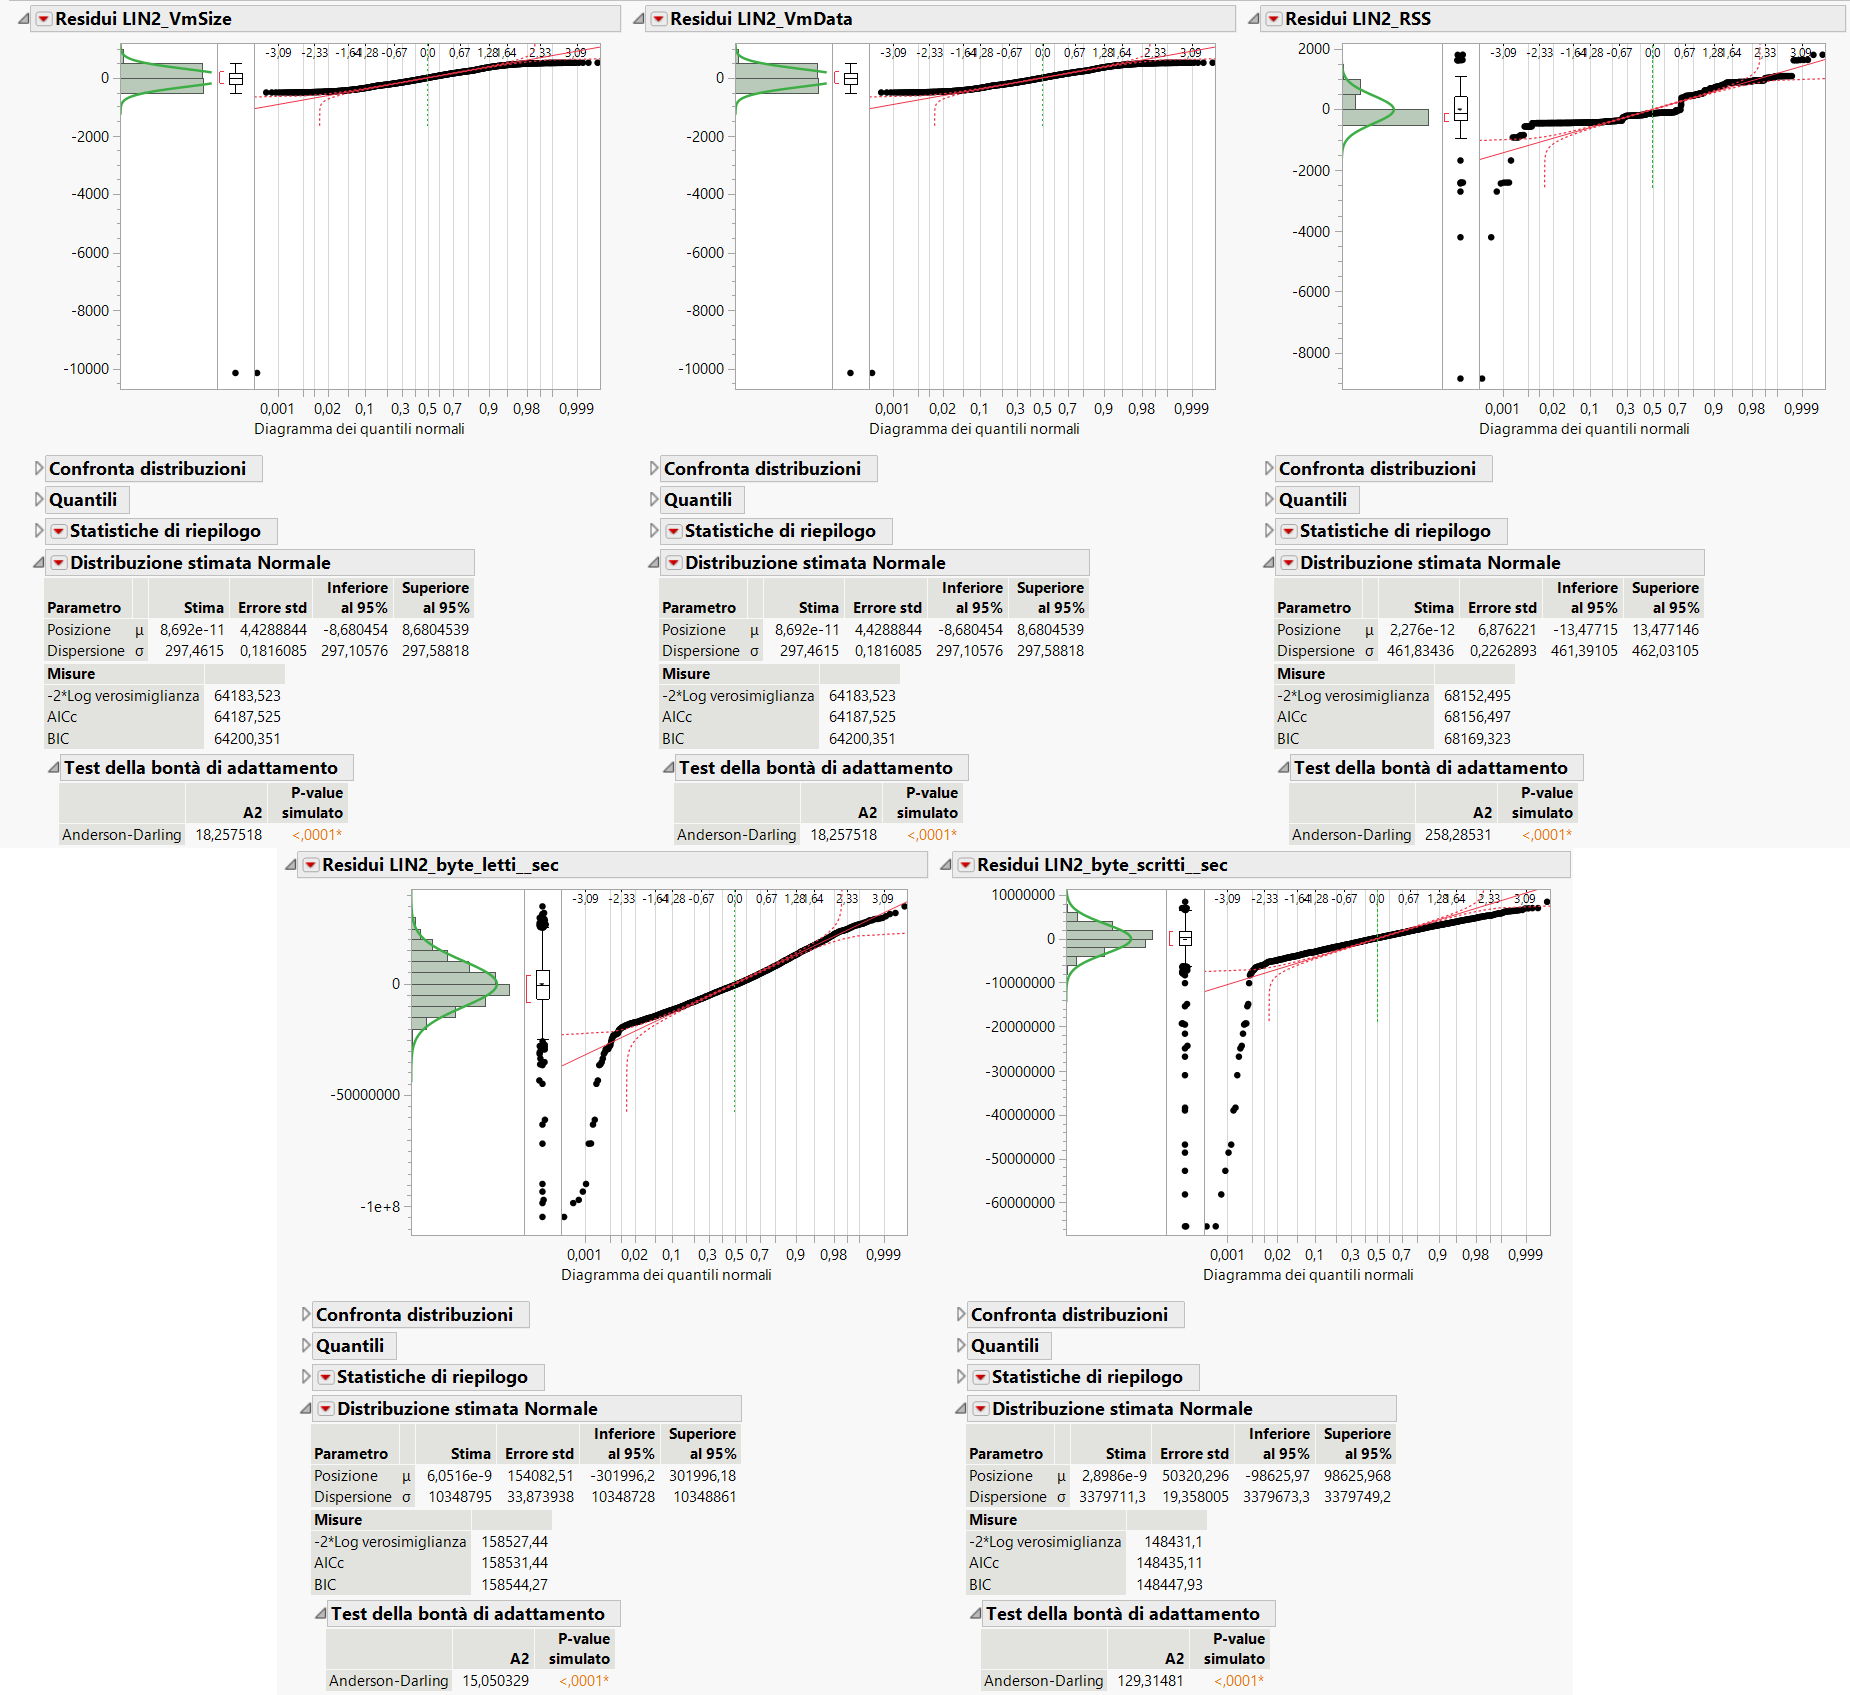
\includegraphics[width=\textwidth]{img/ch4/os2norm.png}
    \caption{Test normalità residui}
    \label{fig:4_os2_traccia}
\end{figure}

\paragraph{LIN2 VmSize}
Il risultato del test di Man Kendall mostra la presenza di un \textit{trend} crescente ($pvalue=0.0$). Il test di Theil-Sen produce una retta:
\begin{equation}
    y = 0.0019 x + 735790.3761
\end{equation}

L'intervallo di confidenza (calcolato al $95\%$) del coefficiente angolare è\\ $(0.0;0.0020)$.


\begin{figure}[H]
    \centering
    \includegraphics[width=\textwidth]{img/ch4/os2.1.pdf}
    \caption{Trend LIN2 VmSize}
\end{figure}

\paragraph{LIN2 VmData}
Il risultato del test di Man Kendall mostra la presenza di un \textit{trend} crescente ($pvalue=0.0$). Il test di Theil-Sen produce una retta:
\begin{equation}
    y = 0.0019 x + 667414.3761
\end{equation}

L'intervallo di confidenza (calcolato al $95\%$) del coefficiente angolare è\\ $(0.0;0.0020)$.

\begin{figure}[H]
    \centering
    \includegraphics[width=\textwidth]{img/ch4/os2.2.pdf}
    \caption{Trend LIN2 VmData}
\end{figure}

\paragraph{LIN2 RSS}
Il risultato del test di Man Kendall mostra la presenza di un \textit{trend} crescente ($pvalue=0.0$). Il test di Theil-Sen produce una retta:
\begin{equation}
    y = 0.0006x + 42384.8545
\end{equation}

L'intervallo di confidenza (calcolato al $95\%$) del coefficiente angolare è\\ $(0.0005;0.0007)$.

\begin{figure}[H]
    \centering
    \includegraphics[width=\textwidth]{img/ch4/os2.3.pdf}
    \caption{Trend LIN2 RSS}
\end{figure}

\paragraph{LIN2 byte letti sec}
Il risultato del test di Man Kendall mostra la presenza di un \textit{trend} crescente ($pvalue=0.0$). Il test di Theil-Sen produce una retta:
\begin{equation}
    y = 114.5535 x + 77733384.2378
\end{equation}

L'intervallo di confidenza (calcolato al $95\%$) del coefficiente angolare è\\ $(112.7335;116.3765)$.


\begin{figure}[H]
    \centering
    \includegraphics[width=\textwidth]{img/ch4/os2.4.pdf}
    \caption{Trend LIN2  byte letti sec}
\end{figure}

\paragraph{LIN2 byte scritti sec}
Il risultato del test di Man Kendall mostra la presenza di un \textit{trend} decrescente ($pvalue=0.0$). Il test di Theil-Sen produce una retta:
\begin{equation}
    y = -0.4886 x + 65693615.5762
\end{equation}

L'intervallo di confidenza (calcolato al $95\%$) del coefficiente angolare è\\ $(-0.9390;-0.0363)$.

\begin{figure}[H]
    \centering
    \includegraphics[width=\textwidth]{img/ch4/os2.5.pdf}
    \caption{LIN2 byte scritti sec}
\end{figure}

\newpage
\subsection{os3}

è possibile notare dal diagramma quantile quantile e dal test di \textit{Anderson-Darlnig} la non normalità delle distribuzioni (\cref{fig:4_os3_traccia}).
Si è quindi proceduto con il test di \textit{Mann Kendall} per verificare la presenza di trend monotoni, e in caso positivo è stato calcolato lo slope con la procedura di \textit{Theil-Sen}.

\begin{figure}[H]
    \centering
    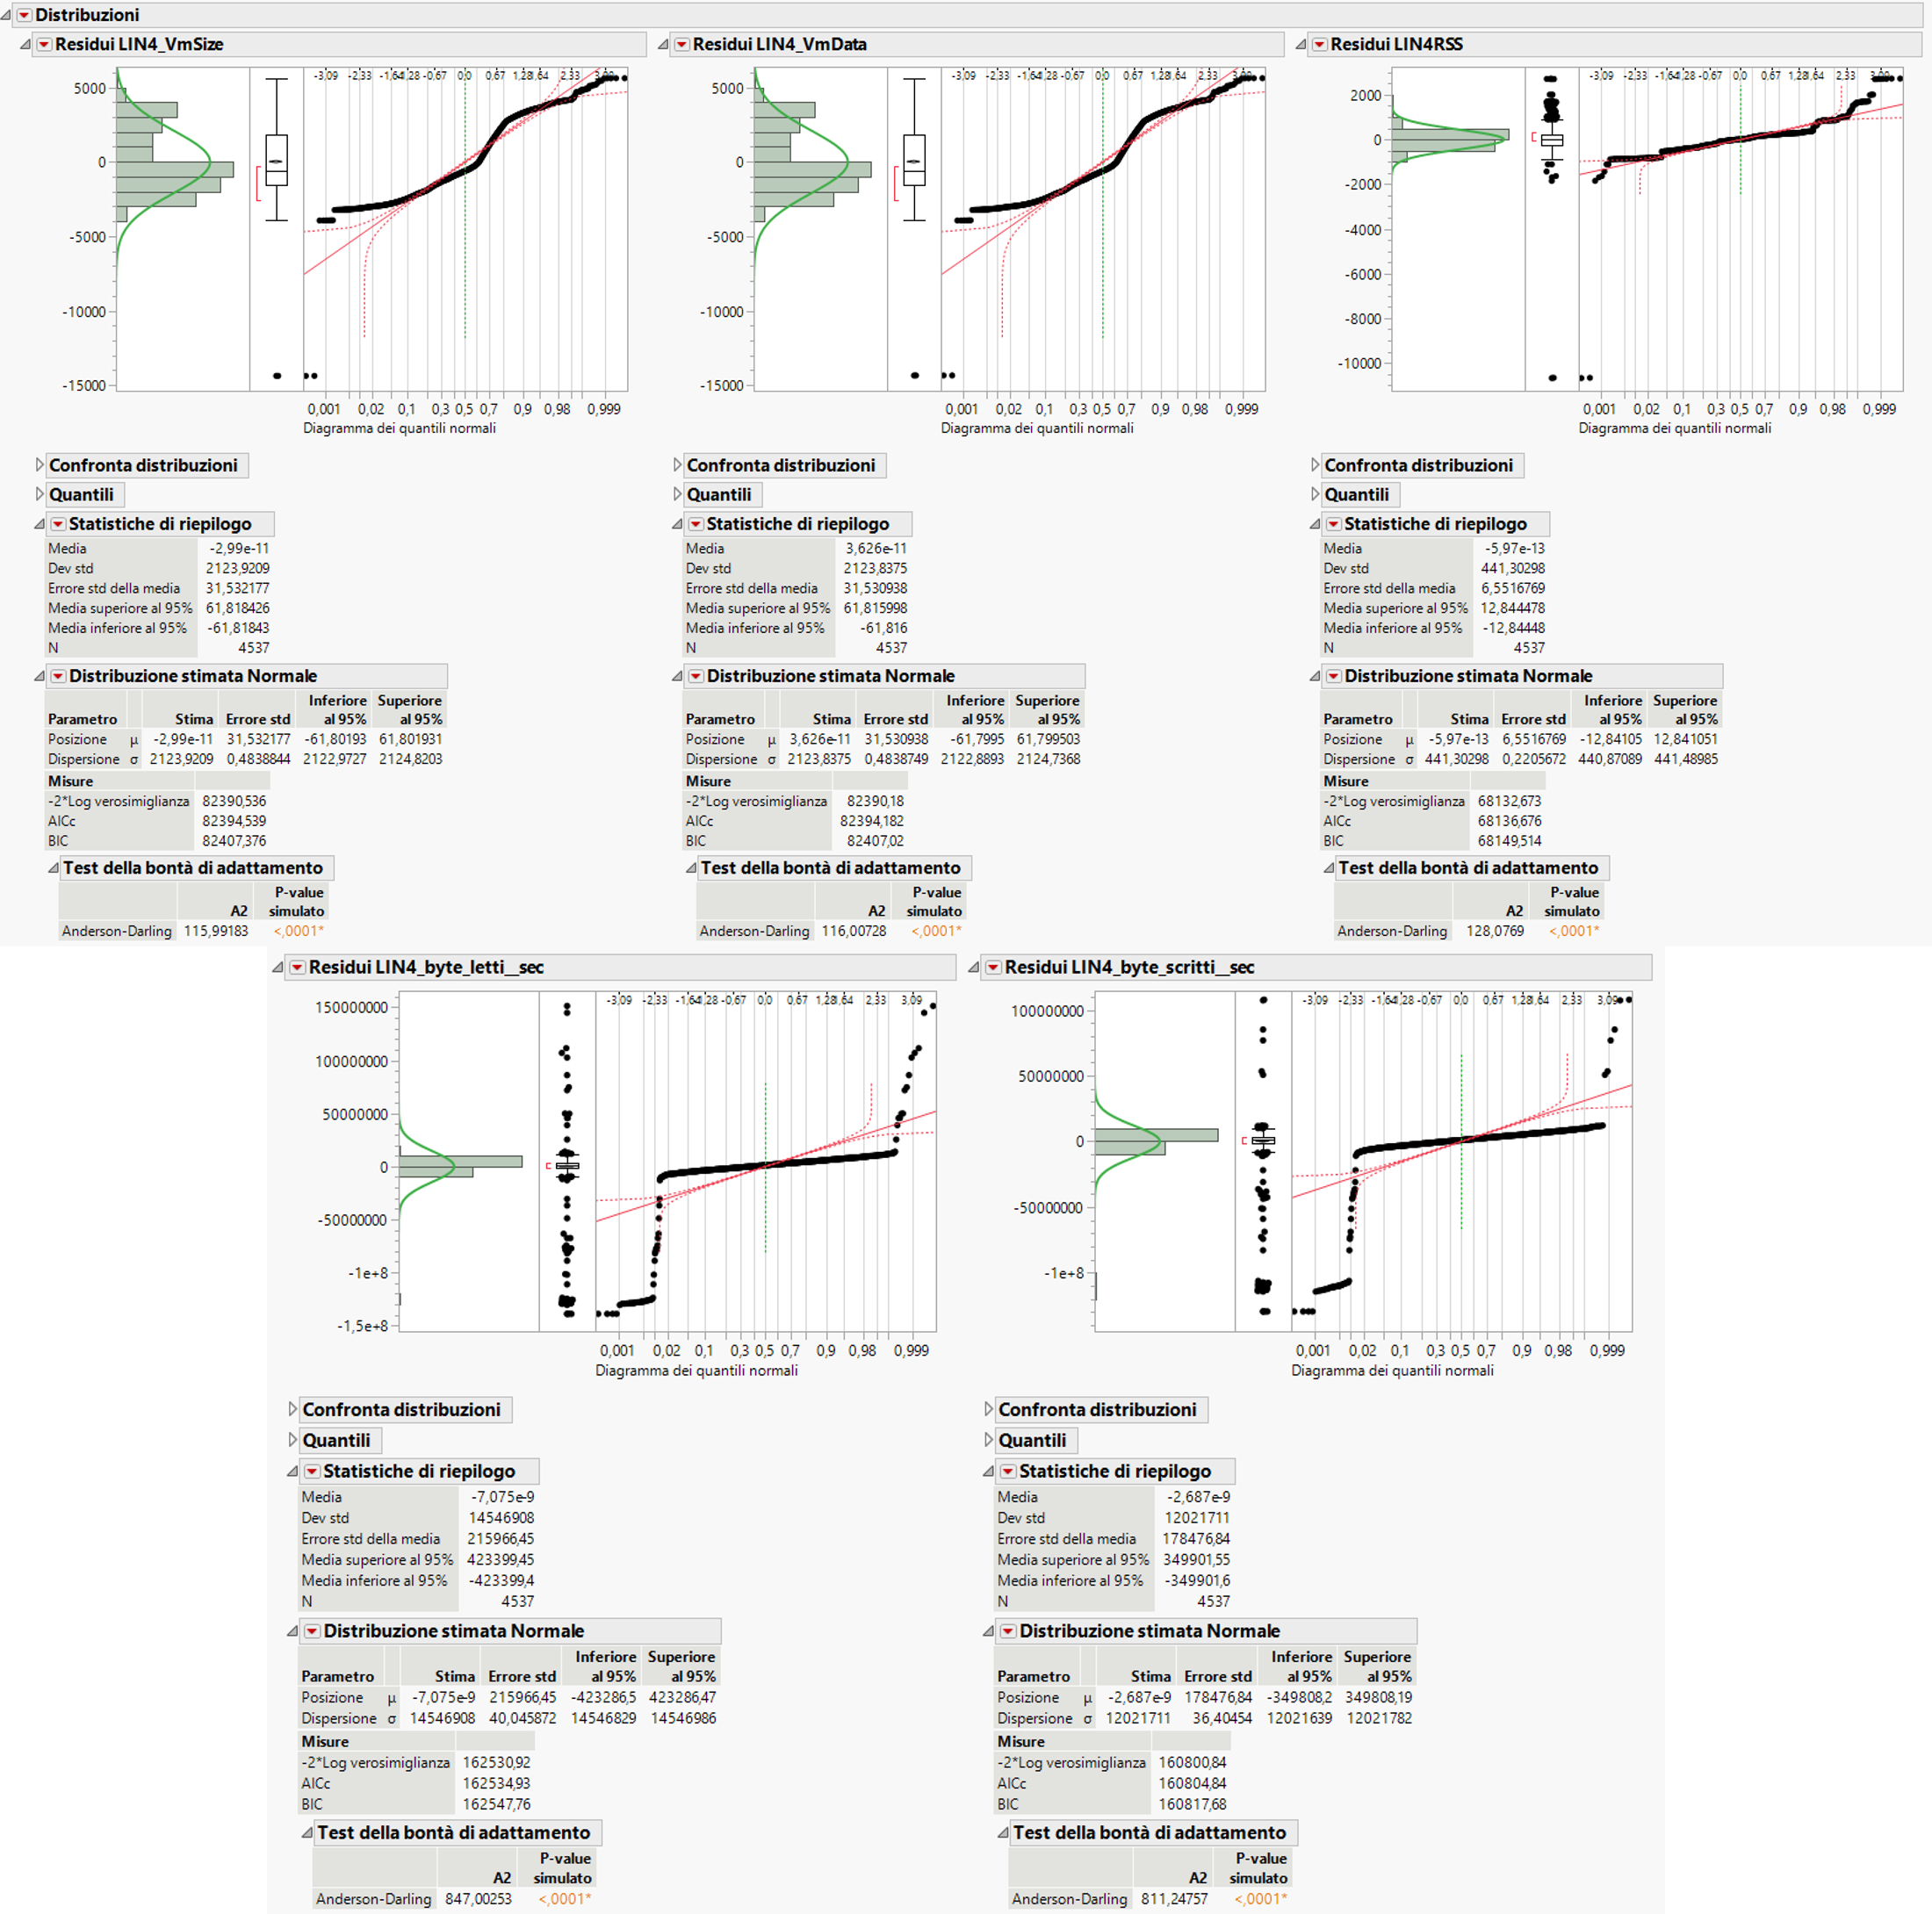
\includegraphics[width=\textwidth]{img/ch4/os3_norm.png}
    \caption{Test normalità residui}
    \label{fig:4_os3_traccia}
\end{figure}

\paragraph{LIN4 VmSize}
Il risultato del test di Man Kendall mostra la presenza di un \textit{trend} crescente ($pvalue=0.0$). Il test di Theil-Sen produce una retta:
\begin{equation}
    y = 0.0216 x + 744373.4861
\end{equation}

L'intervallo di confidenza (calcolato al $95\%$) del coefficiente angolare è\\ $(0.0212;0.0220)$.

\begin{figure}[H]
    \centering
    \includegraphics[width=\textwidth]{img/ch4/os3.1.pdf}
    \caption{LIN4 VmSize}
\end{figure}

\paragraph{LIN4 VmData}
Il risultato del test di Man Kendall mostra la presenza di un \textit{trend} crescente ($pvalue=0.0$). Il test di Theil-Sen produce una retta:
\begin{equation}
    y = 0.0217 x + 675969.4861
\end{equation}

L'intervallo di confidenza (calcolato al $95\%$) del coefficiente angolare è\\ $(0.0212;0.0220)$.

\begin{figure}[H]
    \centering
    \includegraphics[width=\textwidth]{img/ch4/os3.2.pdf}
    \caption{Trend LIN4 VmData}
    \label{fig:ex1_traccia}
\end{figure}

\paragraph{LIN4 RSS}
Il risultato del test di Man Kendall mostra la presenza di un \textit{trend} crescente ($pvalue=0.0$). Il test di Theil-Sen produce una retta:
\begin{equation}
    y = 0.0034 x + 45386.0844
\end{equation}

L'intervallo di confidenza (calcolato al $95\%$) del coefficiente angolare è\\ $(0.0033;0.0035)$.

\begin{figure}[H]
    \centering
    \includegraphics[width=\textwidth]{img/ch4/os3.3.pdf}
    \caption{Trend LIN4 RSS}
\end{figure}

\paragraph{LIN4 byte letti sec}
Il risultato del test di Man Kendall mostra la presenza di un \textit{trend} decrescente ($pvalue=1.0286 \cdot 10^{-7}$). Il test di Theil-Sen produce una retta:
\begin{equation}
    y = -1.9637 x + 141319342.3890
\end{equation}

L'intervallo di confidenza (calcolato al $95\%$) del coefficiente angolare è\\ $(-2.6876;-1.2433)$.

\begin{figure}[H]
    \centering
    \includegraphics[width=\textwidth]{img/ch4/os3.4.pdf}
    \caption{Trend LIN4 byte letti sec}
\end{figure}

\paragraph{LIN4 byte scritti sec}
Il risultato del test di Man Kendall mostra che non è possibile determinare la presenza di un \textit{trend} ($pvalue=0.0539$). Si noti che l'intervallo di confidenza individuato con il test di Theil-Sen $(-1.2588;0.0104)$ include il valore $0$. 


\begin{figure}[H]
    \centering
    \includegraphics[width=\textwidth]{img/ch4/os3.5.pdf}
    \caption{LIN4 byte scritti sec}
\end{figure}

\newpage
\subsection{Confronto tra i sistemi}

\begin{figure}[H]
    \centering
    \includegraphics[width=\textwidth]{img/ch4/os_comp.pdf}
    \caption{Confronto tra \textit{os1}, \textit{os2}, \textit{os3}}
\end{figure}


\begin{itemize}
    \item Memoria Virtuale: dai grafici, si osserva che VMsize e VMdata sono correlati strettamente tra loro , e che in \textit{os1} e \textit{os3} sono presenti trend monotoni crescenti più accentuati, mentre per \textit{os2} c'è sempre un trend crescente ma più lento.
    \item RSS: anche in questo caso tutti i sistemi presentano dei trend monotoni crescenti, con \textit{os2} meno accentuato.
    \item Byte letti: dai risultati ottenuti è possibile notare un trend monotono crescente accentuato su \textit{os2}, mentre per \textit{os1} e \textit{os3}, sono presenti rispettivamente un trend crescente e uno decrescente, entrambi di lieve entità.
    \item Byte scritti: per \textit{os1} e \textit{os3} non è stato rilevato alcun trend, e per os2 esiste un trend monotono decrescente poco accentuato.
\end{itemize}

\newpage
\section{Exercise 3}
Supponendo di avere un limite massimo alla memoria heap di 1 GByte. Rilevare un eventuale trend di consumo dello heap nell'esperimento in figura. Se rilevato il trend, stimare il tempo  in cui lo heap satura (failure prediction).

\subsection{VMres1}
La \cref{fig:4_vmres1_traccia} mostra la non normalità dei residui. Quindi si è proceduto con l'applicazione dei test non parametrici quali \textit{Man-Kendall} per il rilevamento di trend e di \textit{Theil-Sen} per il calcolo dei parametri della retta regressiva.
\begin{figure}[H]
    \centering
    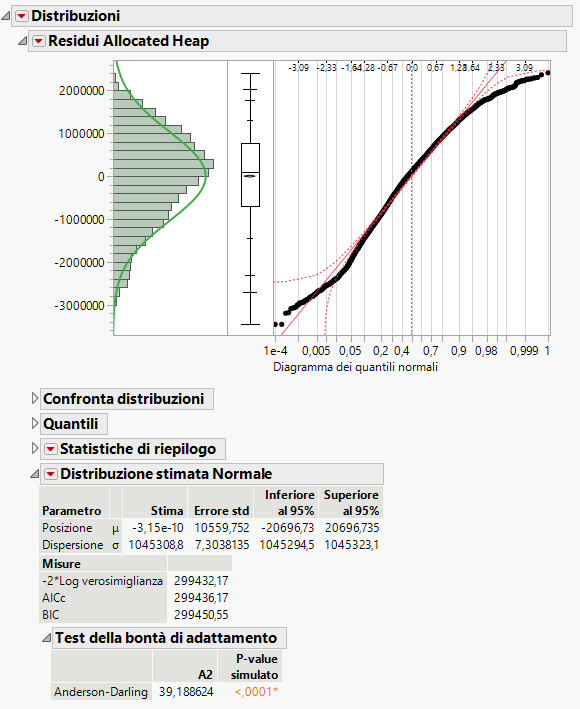
\includegraphics[width=\textwidth]{img/ch4/vm1_norm.png}
    \caption{Normalità residui VMres1}
    \label{fig:4_vmres1_traccia}
\end{figure}


\paragraph{Allocated Heap}
Il risultato del test di Man Kendall mostra la presenza di un \textit{trend} crescente ($pvalue=0.0$). Il test di Theil-Sen produce una retta:
\begin{equation}
    y = 0.6911 x + 6562275.4616
\end{equation}

L'intervallo di confidenza (calcolato al $95\%$) del coefficiente angolare è\\ $(0.5637;0.8178)$.

\begin{figure}[H]
    \centering
    \includegraphics[width=\textwidth]{img/ch4/vmres1.1.pdf}
    \caption{Trend Allocated Heap}
\end{figure}

\subsection{VMres2}
Analogamente a \textit{VMRes1}, anche i residui di \textit{VMRes2} non seguono una distribuione normale (\cref{fig:4_vmres2_traccia}). Pertanto, si è proceduto con l'applicazione di test non parametrici.
\begin{figure}[H]
    \centering
    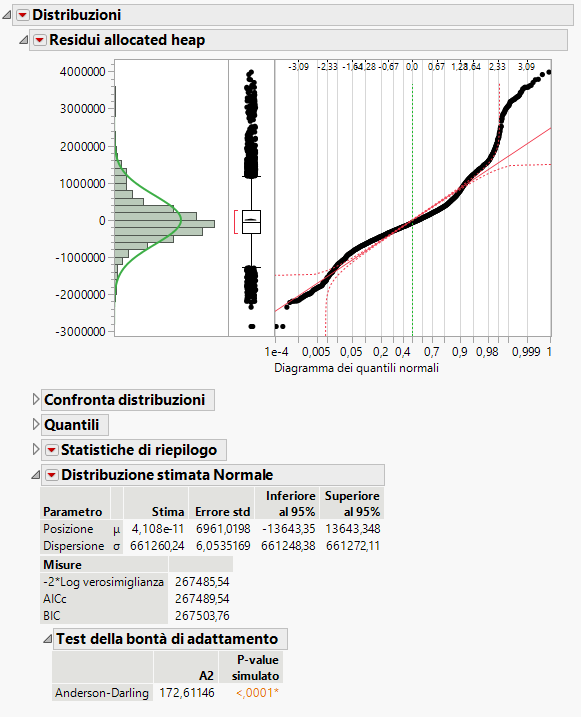
\includegraphics[width=\textwidth]{img/ch4/vm2_norm.png}
    \caption{Normalità residui VMres2}
     \label{fig:4_vmres2_traccia}
\end{figure}

\paragraph{Allocated Heap}

Il risultato del test di Man Kendall mostra la presenza di un \textit{trend} crescente ($pvalue=1.0286 \cdot 10^{-7}$). Il test di Theil-Sen produce una retta:
\begin{equation}
    y = 0.6709 x + 5780180.5633
\end{equation}

L'intervallo di confidenza (calcolato al $95\%$) del coefficiente angolare è\\ $(0.6048;0.7366)$.

\begin{figure}[H]
    \centering
    \includegraphics[width=\textwidth]{img/ch4/vmres2.1.pdf}
    \caption{Trend Allocated Heap}
\end{figure}

\subsection{VMres3}
Infine, anche i residui di \textit{VMRes3} non seguono la distribuzione normale (\cref{fig:4_vmres3_traccia}). Quindi, si è applicato il test \textit{Man-Kendall} per il rilevamento dei \textit{trend}.

\begin{figure}[H]
    \centering
    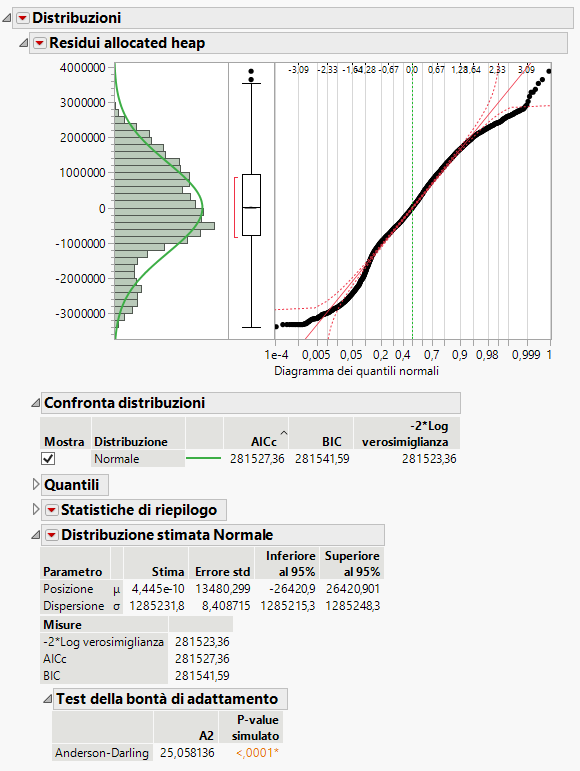
\includegraphics[width=\textwidth]{img/ch4/vm3_norm.png}
    \caption{Normalità residui VMres3}
     \label{fig:4_vmres3_traccia}
\end{figure}

\paragraph{Allocated Heap}

Il risultato del test di Man Kendall mostra la presenza di un \textit{trend} crescente ($pvalue=1.0286 \cdot 10^{-7}$). Il test di Theil-Sen produce una retta:
\begin{equation}
    y = 2.9030 x + 6041585.5564
\end{equation}

L'intervallo di confidenza (calcolato al $95\%$) del coefficiente angolare è\\ $(2.7147;3.0923)$.

\begin{figure}[H]
    \centering
    \includegraphics[width=\textwidth]{img/ch4/vmres3.1.pdf}
    \caption{Trend Allocated Heap}
\end{figure}

\clearpage
\subsection{Failure prediction} 

Dai risultati precedenti è possibile ottenere le rette di regressione relative ai 3 sistemi (riportate in \cref{eq:vm1_regression}, \cref{eq:vm2_regression}, \cref{eq:vm3_regression}), all'interno delle quali basterà imporre $Allocated\_Heap = 1000000000$ per trovare il tempo di saturazione a $1GB$.

\begin{align}
    \label{eq:vm1_regression}
    Allocated\_Heap_1 = 0.6911 \cdot T(s) +6562275.4616 \\ 
    \label{eq:vm2_regression}
    Allocated\_Heap_2 = 0.6709 \cdot T(s) +5780180.5633 \\
    \label{eq:vm3_regression}
    Allocated\_Heap_3 = 2.9030 \cdot T(s) +6041585.5564
\end{align}

Quindi sostituendo i valori numerici, si ottengono i seguenti tempi di saturazione:
\begin{itemize}
    \item VMres1: $ T \approx 45,6 $ anni 
    \item VMres2: $ T \approx 46,9 $ anni
    \item VMres3: $ T \approx 10,8 $ anni
\end{itemize}









